% This work is licensed under the Creative Commons
% Attribution-NonCommercial-ShareAlike 4.0 International License. To view a copy
% of this license, visit http://creativecommons.org/licenses/by-nc-sa/4.0/ or
% send a letter to Creative Commons, PO Box 1866, Mountain View, CA 94042, USA.

\section{Aufgabenblatt 3}
\subsection{Aufgabe 3.1}
Seien $\sigma,\tau$ Stoppzeiten bzgl. der Filtration $(\F_n)_{n\in\N}$ und $\F_\tau$ definiert durch
\begin{align*}
	\F_\tau:=\big\lbrace A\in\A~\big|~\forall n\in\N_0:A\cap\lbrace\tau\leq n\rbrace\in\F_n\big\rbrace
\end{align*}

Dann gilt:
\begin{enumerate}[label=\alph*)]
	\item $\F_\tau$ ist eine $\sigma$-Algebra
	\item $\begin{aligned}
		\sigma\leq\tau\implies\F_\sigma\subseteq\F_\tau
	\end{aligned}$
	\item $\begin{aligned}
		\lbrace\tau\leq\sigma\rbrace\in\F_\tau\cap\F_\sigma
	\end{aligned}$
	\item $\begin{aligned}
		\F_\tau\cap\F_\sigma=\F_{\tau\wedge\sigma}
	\end{aligned}$
\end{enumerate}

\begin{proof}[Beweis von Willi \& Robert.]\enter
	\underline{Zeige a):} Sei $n\in\N_0$ beliebig aber fest.
	\begin{itemize} 
		\item $\Omega\in\F_\tau$, denn $\Omega\in\A$ und 
		\begin{align*}
			\Omega\cap\lbrace\tau\leq n\rbrace=\lbrace\tau\leq n\rbrace \stackrel{\text{SZ}}{\in} \F_n
		\end{align*}
		\item Sei $A \in \F_\tau$. Dann gilt $A^C \in \F_\tau$, denn:
		\begin{align*}
			\lbrace\tau\leq n\rbrace &=\big(\lbrace\tau\leq n\rbrace\cap A\big)\dot{\cup}\big(\lbrace\tau\leq n\rbrace\cap A^C\big)\\
			\implies A^C\cap\lbrace\tau\leq n\rbrace&=\underbrace{\lbrace\tau\leq n\rbrace}_{\stackrel{\text{SZ}}{\in}\F_n}\setminus\big(\underbrace{\lbrace\tau\leq n\rbrace\cap A\big)}_{\stackrel{\text{Vor}}{\in}\F_n}\stackrel{\sigma\text{A}}{\in}\F_n
		\end{align*}
		Alternative: Sei $A \in \F_\tau$
		\begin{align*}
			A^C\cap \lbrace \tau \leq n \rbrace = \left(\underbrace{A}_{\stackrel{\text{Vor.}}{\in} \F_n} \cup \underbrace{\lbrace \tau \leq n \rbrace^C}_{\stackrel{\sigma\text{-Alg}}{\in} \F_n} \right)^C \stackrel{\sigma\text{-Alg}}{\in}\F_n
		\end{align*}

		\item Sei $(A_i)_{i\in\N}\subseteq\F_\tau$. 
		Dann gilt $\bigcup\limits_{i\in\N} A_i  \in \F_\tau$, denn:\\
		Offenbar ist $\bigcup\limits_{i\in\N} A_i  \in\A$ und nach Voraussetzung gilt $A_i\in\A$ und\\ $A_i\cap\lbrace\tau\leq n\rbrace\in\F_n~\forall i\in\N_0$. 
		Folglich gilt:
		\begin{align*}
			\underbrace{\bigcup\limits_{i=1}^{\infty} \Big (A_i \cap \{\tau \leq n\} \Big )}_{\stackrel{\sigma\text{A}}{\in} \F_n} = \left( \bigcup\limits_{i=1}^{\infty} A_i \right)\cap \{\tau \leq n\} \implies  \bigcup\limits_{i=1}^{\infty} A_i \in \F_\tau
		\end{align*}
	\end{itemize}

	\underline{Zeige b):}\\
	Sei $A\in\F_\sigma$. 
	Dann ist $A\in\A$ und $A\cap\lbrace\sigma\leq n\rbrace\in\F_n\forall n\in\N_0.$ 
	Also gilt:
	\begin{align*}
		A \cap \lbrace\tau \leq n\rbrace
		\overset{}=
		\big(A \cap\lbrace\tau \leq n\rbrace\big)\cap\underbrace{\lbrace\sigma\leq\tau\rbrace}_{\stackeq{\text{Vor.}}\Omega}
		=\underbrace{A\cap\lbrace\sigma\leq n\rbrace}_{\stackrel{\text{Vor}}{\in}\F_n}\cap\underbrace{\lbrace\tau\leq n\rbrace}_{\stackrel{\text{SZ}}{\in}\F_n} \stackrel{\sigma\text{A}}{\in} \F_n\\ \quad \forall n \in \N_0
		\implies A\in\F_\tau
	\end{align*}

	\underline{Zeige c):}\\
	Es ist ausreichend folgende zwei Aussagen zu zeigen:
	\begin{align*}
		\lbrace \tau \leq \sigma\rbrace &\cap \lbrace \tau \leq n\rbrace \in \F_n &(\ast)&\\
		\lbrace \tau \leq \sigma\rbrace &\cap \lbrace \sigma \leq n\rbrace \in \F_n &(\ast\ast)& \\
	\end{align*}

	Zu $(\ast)$:
	\begin{align*}
		&\lbrace \tau \leq \sigma\rbrace \cap \lbrace \tau \leq n\rbrace\\
		=&\lbrace \tau \leq \min\{\sigma, n\}\rbrace  \\
		=&\lbrace \tau \leq \min\{\sigma, n\}, \sigma \geq n\rbrace \cup 
		\lbrace \tau \leq \min\{\sigma, n\}, \sigma < n\rbrace \\
		=&\underbrace{\lbrace \tau \leq n\rbrace}_{\in \F_n} \cup
		\underbrace{\lbrace \tau \leq \sigma, \sigma < n\rbrace}_{\in \F_\sigma \subset \F_n} \in \F_n \\
	\end{align*}

	Zu $(\ast\ast)$:
	Verläuft ähnlich wie der letzte Schritt in $(\ast)$:
	\begin{align*}
		&\lbrace \tau \leq \sigma\rbrace \cap \lbrace \sigma \leq n\rbrace \\
		&=\underbrace{\lbrace \tau \leq \sigma, \sigma \leq n\rbrace}_{\F_\sigma \subset F_n} \in F_n \\
	\end{align*}
	
	\textbf{Alternative vom Prof.:}\\
	Zu zeigen: $\lbrace\sigma\leq\tau\rbrace\in\F_\tau\cap\F_\sigma$
	\begin{align*}
		\lbrace\sigma\leq\tau\rbrace\cap\lbrace\tau\leq n\rbrace
		&=\bigcup\limits_{k=0}^n\underbrace{\lbrace \sigma=k\rbrace}_{\in\F_n}\cap\underbrace{\lbrace k\leq\tau\rbrace}_{\in\F_n}\cap\underbrace{\lbrace\tau\leq n\rbrace}_{\in\F_n}\in\F_n &\forall n\in\N_0\\
		\lbrace\sigma\leq\tau\rbrace\cap\lbrace\sigma\leq n\rbrace
		&=\bigcup\limits_{k=0}^n\underbrace{\lbrace\sigma=k\rbrace}_{\in \F_n}\cap\underbrace{\lbrace k\leq n\rbrace}_{\in\F_n}\in\F_n &\forall n\in\N_0\\
		&\implies\lbrace\sigma\leq\tau\rbrace\in\F_n
	\end{align*}

	\underline{Zeige d):}\
	\begin{itemize}
		\item Zeige ``$\subseteq$'':
		Sei $A\in\F_\tau\cap\F_\sigma$. Dann ist $A\in\A$ und
		\begin{align*}
			\big(A\cap\lbrace\tau\leq n\rbrace\big),\big(A\cap\lbrace\sigma\leq n\rbrace\big)\in\F_n\qquad\forall n\in\N_0
		\end{align*}
		Da $\F_n$ eine $\sigma$-Algebra ist, ist auch die Vereinigung enthalten:
		\begin{align*}
			&\big(A\cap\lbrace\tau\leq n\rbrace\big)\cup\big(A\cap\lbrace\sigma\leq n\rbrace\big)\in\F_n\\
			&\implies
			\big(A\cap\lbrace\tau\leq n\rbrace\big)\cup\big(A\cap\lbrace\sigma\leq n\rbrace\big)
			&=&A\cap\big(\lbrace\tau\leq n\rbrace\cup\lbrace\sigma\leq n\rbrace\big)\\
			&&=&A\cap\lbrace\tau\wedge\sigma\leq n\rbrace\in\F_n\\
			&\implies A\in\F_{\sigma\wedge\tau}\implies \F_\tau\cap\F_\sigma\subseteq\F_{\tau\wedge\sigma}
		\end{align*}

		\item Zeige ``$\supseteq$'':
		\begin{align*}
			\tau\wedge\sigma\stackrel{\text{Def}}{\leq}\tau,\sigma\stackrel{\text{(b)}}{\implies}\F_{\sigma\wedge\tau}\subseteq\F_\tau,\F_\sigma\implies\F_{\tau\wedge\sigma}\subseteq\F_\tau\cap\F_\sigma
		\end{align*}
	\end{itemize}
\end{proof}

\begin{proof}[Beweis von Henrik.]
	\underline{Zeige a):}\
	\begin{itemize} 
		\item z.z.:$\emptyset \in \F_\tau$
		\begin{equation*}
			\emptyset \in \A \text{ und } \emptyset \in \F_n\  \forall n \in \N_0 \implies \emptyset \cap \{\tau \leq n\} \in \F_n
		\end{equation*}
		\item z.z.: $A \in \F_\tau \implies A^C \in \F_\tau$\\
		Sei $A \in \F_\tau$, d.h.:
		\begin{align*}
			&{}\qquad \quad  A \cap \{\tau \leq n\} \in \F_n
			 &\forall n \in \N\\
			&\implies	A^C \cup \{\tau > n\} \in \F_n 
			 &\forall n \in \N\\
			&\implies 	\left(	A^C \cup \{\tau > n\}\right) \cap \{\tau \leq n\} \in \F_n
			 & \forall n \in \N\\
			& \iff \left(	A^C \cap \{\tau \leq n\}\right) \cup \underbrace{\big ( \{\tau > n\}\cap\{\tau \leq n\} \big )}_{= \emptyset} \in \F_n 
			 & \forall n \in \N\\
			&\implies A^C \cap \{\tau \leq n\} \in \F_n
			 & \forall n \in \N
		\end{align*}
	
		\item z.z.: Sei $A_1, A_2,\dots \in \F_\tau \implies \bigcup\limits_{i=1}^{\infty} A_i  \in \F_\tau$
		\begin{equation*}
			\underbrace{\bigcup\limits_{i=1}^{\infty} \Big (A_i \cap \{\tau \leq n\} \Big )}_{\in \F_n} = \left( \bigcup\limits_{i=1}^{\infty} A_i \right)\cap \{\tau \leq n\} \implies  \bigcup\limits_{i=1}^{\infty} A_i \in \F_\tau
		\end{equation*}
	\end{itemize}

	\underline{Zeige b):}
	% @Henrik: Ich habe mir mal erlaubt, deinen Beweis zu korrigieren. Kannst du gern auch beliebig abändern.
	%PS: Ich hatte dir sogar geschrieben, dass du \sigma und \tau vertauscht hast :D
	\begin{align*}
		&{}\qquad \quad  A \cap \{\sigma \leq n\}  \in \F_n \quad \forall n \in \N\\
		&\implies A \cap \{\tau \leq n\} \cap \{\tau \leq n\} = A \cap \underbrace{ \{\tau \vee \sigma \leq n\}}_{ \overset{\sigma \leq \tau}{=} \{\sigma \leq n\} } \in \F_n \quad \forall n \in \N\\
		&\implies A \in \F_\tau \\
	\end{align*}

	%\underline{Zeige c):}
	%TODO broken proof
	%z.z.: $\ \{\tau \leq \sigma\} \in \F_\tau \cap \F_\sigma$\\
	%Wir wissen $\{\tau \leq n\} \in \F_\tau$ und  $\{\sigma \geq n\} \in \F_\sigma$ (siehe Aufgabe 2.4 ). Damit gilt: $\{\tau \leq n\} \cap \{\sigma \geq n\} = \{\tau \leq \sigma\} $ ist Element von $\F_\tau \cap \F_\sigma$.\\

	%\underline{Zeige d):}
	%TODO broken proof
	%\begin{align*}
	%&{} \qquad \quad  A \cap \{\tau \leq n\}\in \F_n \text{ und } A \cap\{\sigma \leq n\}\in \F_n &\forall n \in \N\\
	%&\iff  A \cap \{\tau \leq n\} \cap \{\sigma \leq n\}\in \F_n &\forall n \in \N \\
	%&\iff  A \cap \{\tau \land \sigma \leq n\} \in \F_n &\forall n \in \N\\
	%&\iff A \in \F_{\tau \land \sigma} \\
	%\end{align*}
\end{proof}

\subsection{Aufgabe 3.2}
Sei $(X_i)_{i\in I}$ eine Folge von Zufallsvariablen und $\phi:[0,\infty)\to\R$ eine konvexe, wachsende Funktion mit 
\begin{align*}
	\frac{\phi(x)}{x}\stackrel{x\to+\infty}{\longrightarrow}+\infty
\end{align*}
(zum Beispiel $\phi(x):=|x|^p\mit p>1$.) Dann gilt:
\begin{align*}
	\sup\limits_{i\in I}\E\Big[\phi\big(|X_i|\big)\Big]<\infty\implies(X_i)_{i\in I}\text{ ist ggi}
\end{align*}

\begin{proof}
	Sei also das Supremum beschränkt.\nl
	\underline{Fall 1: $\phi(0)=0$}\\
	Es gilt $\frac{\phi(a)}{a}\leq\frac{\phi(b)}{b}$ für $a\leq b$, wegen Konvexität. %TODO WARUM? ALSO FORMAL?

	Zu zeigen:
	\begin{align*}
		\lim\limits_{R\to\infty}\underbrace{\sup\limits_{i\in I}
		\E\Big[|X_i|\cdot\indi_{\lbrace |X_i|\geq R\rbrace}\Big]}_{:=\rho(R)}=0
	\end{align*}
	Aus obiger Ungleichung folgt mit $b = |X_i| \geq R = a$:
	\begin{align}\label{eq2}\tag{$\ast$}
		b \leq \phi(b) \cdot \frac{a}{\phi(a)}
	\end{align}
	Es gilt
	\begin{align*}
		\E\Big[|X_i|\cdot\indi_{\lbrace |X_i|\geq R\rbrace}\Big]
		\overset{\eqref{eq2}}&{\leq}
		\E\bigg[\phi(|X_i|)\cdot\frac{R}{\phi(R)}\cdot\indi_{\lbrace |X_i|\geq R\rbrace}\bigg]\\
		&=\frac{R}{\phi(R)}\cdot\E\Big[\phi(|X_i|)\cdot\indi_{\lbrace |X_i|\geq R\rbrace}\Big]\\
		&\leq\frac{R}{\phi(R)}\cdot\E\Big[\phi(|X_i|)\Big]\\
		\overset{\text{sup}}&{\leq}
		\frac{R}{\phi(R)}\cdot\sup_{i\in I}\E\Big[\phi(|X_i|)\Big]\\
	\end{align*}
	und daraus folgt durch Bildung des Grenzwertes auf beiden Seiten:
	\begin{align*}
		\lim\limits_{R\rightarrow \infty}\rho(R)
		&=\lim\limits_{R\rightarrow \infty} \E\Big[|X_i|\cdot\indi_{\lbrace |X_i|\geq R\rbrace}\Big] \\
		&\leq 
		\underbrace{\lim\limits_{R\rightarrow \infty}\frac{R}{\phi(R)}}_{\stackrel{\text{Vor.}}{\longrightarrow} 0}\cdot\underbrace{\sup_{i\in I}\E\Big[\phi(|X_i|)\Big]}_{\stackrel{\text{Vor}}{\leq} \infty}\\
		&=0
	\end{align*}
	
	Also ist $(X_i)_{i\in I}$ ggi.\nl
	\underline{Fall 2: $\phi(0)=r\in\R\setminus\lbrace0\rbrace$}\\
	Dann setze
	\begin{align*}
		\tilde{\phi}:[0,\infty)\to\R,\qquad\tilde{\phi}(x):=\phi(x)-r\qquad\forall x\in[0,\infty)
	\end{align*}
	Dann gilt $\tilde{\phi}(0)=0$ und außerdem ist $\tilde{\phi}$ offenbar eine konvexe, monoton wachsende Funktion mit
	\begin{align*}
		\frac{\tilde{\phi}(x)}{x}\stackrel{x\to+\infty}{\longrightarrow}+\infty.
	\end{align*}
	Somit wende Fall 1 auf $\tilde{\phi}$ an. Dann folgt die Behauptung.
\end{proof}

\subsection{Aufgabe 3.3}
Sei $(X_n)_{n\in\N}$ der asymmetrische einfache Random Walk mit $\P(\xi_1=1)=p$ und $\P(\xi_1=-1)=q$, vgl. Aufgabenblatt 2, Aufgabe 2.
\begin{enumerate}[label=\alph*)]
	\item Definiere für $A,B\in\N$ durch
	\begin{align*}
		\tau_A:=\inf\big\lbrace n\in\N_0:X_n=A\big\rbrace,\qquad \tau_B:=\inf\limits\big\lbrace n\in\N_0:X_n=-B\big\rbrace
	\end{align*}
	die ersten Treffzeiten von $A$ und $-B$.\\
	Berechnen Sie $\P[\tau_A<\tau_B]$.
	\item Zeige mit Hilfe einer geeigneten Maximalungleichung im Fall $q>p$:
	\begin{align}\label{eqAufgabe3bObere}
		\P\left[\sup\limits_{n\in\N_0} X_n\geq k\right]\leq\left(\frac{p}{q}\right)^k
	\end{align}
	und 
	\begin{align}\label{eqAufgabe3bUntere}
		\E\left[\sup\limits_{n\in\N_0} X_n\right]\leq\frac{q}{q-p}
	\end{align}
\end{enumerate}

\begin{proof}
	\underline{Zu a):}
	\begin{align*}
		a:=\P\big[ X\text{ erreicht }A\text{ vor }-B\big]=\P\big[\tau_A\leq\tau_B\big]
	\end{align*}
	Der asymmetrische Random Walk ist allerdings kein Martingal (wie der symmetrische Random Walk). 
	Wir betrachten also das Martingal vom Aufgabenblatt 2 Aufgabe 2:
	\begin{align*}
		Y_n := \left(\frac{q}{p}\right)^{X_n}
	\end{align*}
	Wir haben bereits bewiesen, dass $Y$ Martingal ist. 
	Außerdem gilt für\\
	$\tau=\tau_A\wedge\tau_B$ die Abschätzung
	\begin{align*}
		\big|Y_{\tau\wedge n}\big|\leq
		\left\lbrace\begin{array}{cl}
			\left(\frac{q}{p}\right)^{\max\lbrace A,B\rbrace}, &\falls q>p\\
			1, &\falls q\leq p
		\end{array}\right..
	\end{align*}
	Somit folgt aus Theorem 3.3 ($\tau$ endlich analog zur Vorlesung):
	\begin{align*}
		\E\big[Y_\tau\big]=\E\big[Y_0\big]=1
	\end{align*}
	Andererseits: 
	\begin{align*}
		1&=\E\big[Y_\tau\big]\\
		&=\E\Big[\underbrace{Y_{\tau_A}}_{=\left(\frac{q}{p}\right)^A}\cdot\indi_{\lbrace\tau_A<\tau_B\rbrace}+\underbrace{Y_{\tau_B}}_{=\left(\frac{q}{p}\right)^{-B}}\cdot\indi_{\lbrace\tau_A>\tau_B\rbrace}\Big]\\
		&=\left(\frac{q}{p}\right)^A\cdot\P\big(\tau_A<\tau_B\big)+\left(\frac{q}{p}\right)^{-B}\cdot\P\big(\tau_A>\tau_B\big)\\
		&=\left(\frac{q}{p}\right)^A\cdot a+ \left(\frac{q}{p}\right)^{-B}\cdot(1-a)\\
		&=a\cdot\left(\left(\frac{q}{p}\right)^A - \left(\frac{p}{q}\right)^{-B}\right)+ \left(\frac{q}{p}\right)^{-B}\\
		&\implies
		a=\frac{1-\left(\frac{q}{p}\right)^{-B}}{\left(\frac{q}{p}\right)^A-\left(\frac{q}{p}\right)^{-B}}
	\end{align*}
	und somit:
	\begin{align*}
		\P\big(X\text{ trifft }+A\text{ vor }-B\big)
		=\frac{1-\left(\frac{q}{p}\right)^{-B}}{\left(\frac{q}{p}\right)^A-\left(\frac{q}{p}\right)^{-B}}
		\overset{\text{Prof}}=
		\frac{\left(\frac{1}{p}-1\right)^B-1}{\left(\frac{1}{p}-1\right)-1}
	\end{align*}

	\underline{Zu b), zeige \eqref{eqAufgabe3bObere}:}
	\begin{align*}
		\P\left(\sup\limits_{n\in \N_0} X_n \geq k\right)
		 \overset{q>p}&{=}
		\P\left(\sup\limits_{n\in \N_0} Y_n \geq \left(\frac{q}{p}\right)^k\right) \\
		&=\P\left(\max\limits_{0\leq n\leq N} Y_n \geq \left(\frac{q}{p}\right)^k\right) \\
		\overset{\text{Max-Ung.}}&{\leq}
		\frac{1}{\left(\frac{q}{p}\right)^k}\cdot\E\left[Y_N^+\right] \\
		&=\left(\frac{p}{q}\right)^k\E\left[Y_N^+\right] \\
		\overset{\text{pos.}}&{=}
		\left(\frac{p}{q}\right)^k\underbrace{\E\left[Y_N\right]}_{=1} \\
		%&\stackeq{\text{bekannt}}
		%\frac{1}{\left(\frac{q}{p}\right)^k}\cdot1 \\
		&=\left(\frac{p}{q}\right)^k
	\end{align*}

	\underline{Zu b), zeige \eqref{eqAufgabe3bUntere}:}
	\begin{align*}
		\E\left[\sup\limits_{n\in \N_0}X_n\right] 
		&= \sum\limits_{k=0}^\infty k\cdot \P\left[\sup\limits_{n\in \N_0}X_n = k\right] \\
		&= \sum\limits_{k=0}^\infty k\cdot\left( \P\left[\sup\limits_{n\in \N_0}X_n \geq k\right] - \P\left[\sup\limits_{n\in \N_0}X_n \geq k+1\right]\right)\\
		&= \sum\limits_{k=0}^\infty k\cdot\P\left[\sup\limits_{n\in \N_0}X_n \geq k\right] - \sum\limits_{k=0}^\infty k \cdot \P\left[\sup\limits_{n\in \N_0}X_n \geq k+1\right]\\
		&= \sum\limits_{k=1}^\infty k\cdot\P\left[\sup\limits_{n\in \N_0}X_n \geq k\right] - \sum\limits_{k=1}^\infty (k-1) \cdot \P\left[\sup\limits_{n\in \N_0}X_n \geq k\right]\\
		&= \sum\limits_{k=1}^\infty\underbrace{\big(k - (k-1)\big)}_{=1} \cdot \P\left[\sup\limits_{n\in \N_0}X_n \geq k\right]\\
		&= \sum\limits_{k=1}^\infty \P\left[\sup\limits_{n\in \N_0}X_n \geq k\right]\\
		\overset{\eqref{eqAufgabe3bObere}}&{\leq}\sum\limits_{k=1}^\infty \left(\frac{p}{q}\right)^k\\
		\overset{q>p}&{=}\frac{1}{1-\left(\frac{p}{q}\right)^k} \\
		&= \frac{q}{q-p}
	\end{align*}
\end{proof}

\subsection{Aufgabe 3.4}
Zeige mit Hilfe der Jensenschen Ungleichung
\begin{align}\label{eqJensenscheUngleichung}\tag{Jensen}
	f\big(\E[X]\big)\leq\E\big[f(X)\big]\qquad\forall X\text{ integrierbar und $f$ konvex},
\end{align}
dem Martingalkonvergenzsatz in $L_1$ und Doob's Maximalungleichung den Konvergenzsatz für $L^p$-beschränkte Martingale:

\begin{theorem}[Konvergenzsatz für $L^p$-beschränkte Martingale]\enter
	Sei $p>1,B>0$ und $(M_n)_{n\in\N_0}$ ein Martingal mit 
	\begin{align*}
		\E\left[|M_n|^p\right]\leq B<\infty.
	\end{align*}
	Dann existiert eine Zufallsvariable $M_\infty$ mit $\E\left[|M_\infty|^p\right]\leq B$ so, dass
	\begin{align*}
		\P\left[\limn M_n=M_\infty\right]=1
		\qquad\text{und}\qquad
		\limn\big\Vert M_n-M_\infty\big\Vert=0
	\end{align*}
\end{theorem}

\begin{proof}
	Wir haben gegeben, dass gilt
	\begin{align*}
		\sup\limits_{n\in\N_0} \E\left[|M_n|^p\right] \leq B < \infty
	\end{align*}
	Daher gilt nach Theorem 4.4. bzw. Aufgabe 2, dass $M_n$ ggi. ist.
	Mit Theorem 4.6. folgt gleich:
	\begin{align*}
		\exists M_\infty \in L^1 : \E\left[|M_n - M_\infty\right]\stackrel{n\rightarrow \infty}{\longrightarrow} 0
	\end{align*}
	Nun betrachten wir die folgende Ungleichung, die nach Doob's Maximalungleichung gilt:
	\begin{align*}
		\P\left[\max\limits_{j\leq n} |M_n - M_\infty| \geq r\right] \leq \frac{1}{r} \E\left[|M_n-M_\infty|\right]
	\end{align*}
	Als nächstes brauchen wir ein Argument, um später den Limes in das linke Wahrscheinlickeitsmaß ziehen zu können. 
	Dazu ist es ausreichend die Monotonie der gemessenen Menge nachzuweisen. 
	Die Mengen
	\begin{align*}
		A_n:&=\lbrace \omega : \max\limits_{j\leq n} |M_j(\omega) - M_\infty(\omega)| \geq r\rbrace \\
		&=\bigcup\limits_{j\leq n}\lbrace \omega : |M_j(\omega) - M_\infty(\omega)| \geq r\rbrace
	\end{align*}
	sind offensichtlich monoton wachsend in $n$. 
	Dies kann man zusätzlich in Skizze \ref{AbbUEProzess} sehen.
	Außerdem brauchen wir noch die triviale Inklusion
	\begin{align*}
		\lbrace \omega : |M_n(\omega) - M_\infty(\omega)| \geq r\rbrace
		&\subset \lbrace \omega : \max\limits_{j\leq n} |M_j(\omega) - M_\infty(\omega)| \geq r\rbrace \\
		&=\bigcup\limits_{j\leq n}\lbrace \omega : |M_j(\omega) - M_\infty(\omega)| \geq r\rbrace
	\end{align*}
	Nun können wir endlich folgern:
	\begin{align*}
		\P\left[\lim\limits_{n\rightarrow\infty}|M_n-M_\infty| \geq r\right] 
		\overset{\text{Mono.}}&{\leq}
		\P\left[\lim\limits_{n\rightarrow\infty}\bigcup\limits_{j\leq n}|M_n-M_\infty| \geq r\right]  \\
		\overset{\text{s.o.}}&=\P\left[\lim\limits_{n\rightarrow\infty}\max\limits_{j\leq n}|M_n-M_\infty| \geq r\right]  \\
		\overset{\text{stetig}}&=\lim\limits_{n\rightarrow\infty}\P\left[\max\limits_{j\leq n}|M_n-M_\infty| \geq r\right]  \\
		\overset{\text{Max-Ungl.}}&{\leq}\lim\limits_{n\rightarrow\infty}\frac{\E\left[|M_n-M_\infty|\right]}{r}  \\
		\overset{L^1-\lim}&= 0 \qquad \forall r\geq 0
	\end{align*}
	Nun können wir die erste Aussage folgern
	\begin{align*}
		\P[\lim\limits_{n\rightarrow\infty}M_n \neq M_\infty]
		&=\P\left[\bigcup\limits_{k\in\N}\left\lbrace\lim\limits_{n\rightarrow\infty}|M_n-M_\infty| \geq \frac{1}{k}\right\rbrace\right] \\
		\overset{\sigma-\text{Add.}}&{\leq} \sum\limits_{k\in\N}
		\P\left[\lim\limits_{n\rightarrow\infty}|M_n-M_\infty| \geq \frac{1}{k}\right] \\
		&\stackrel{\text{s.o.}}{\leq} 0
	\end{align*}
	Also ist $M_\infty$ fast sicher der Grenzwert von $M_n$. 
	Nun folgt der Rest sehr wie im Beweis vom Professor.
\end{proof}

\begin{figure}[H]
	\begin{center}
		\caption{Die drei wesentlichen Fälle die bei einem beliebigen Schritt $n\rightarrow n+1$ des Prozesses $Z_i:=M_i(\omega)-M_\infty(\omega)$ eintreten können}
		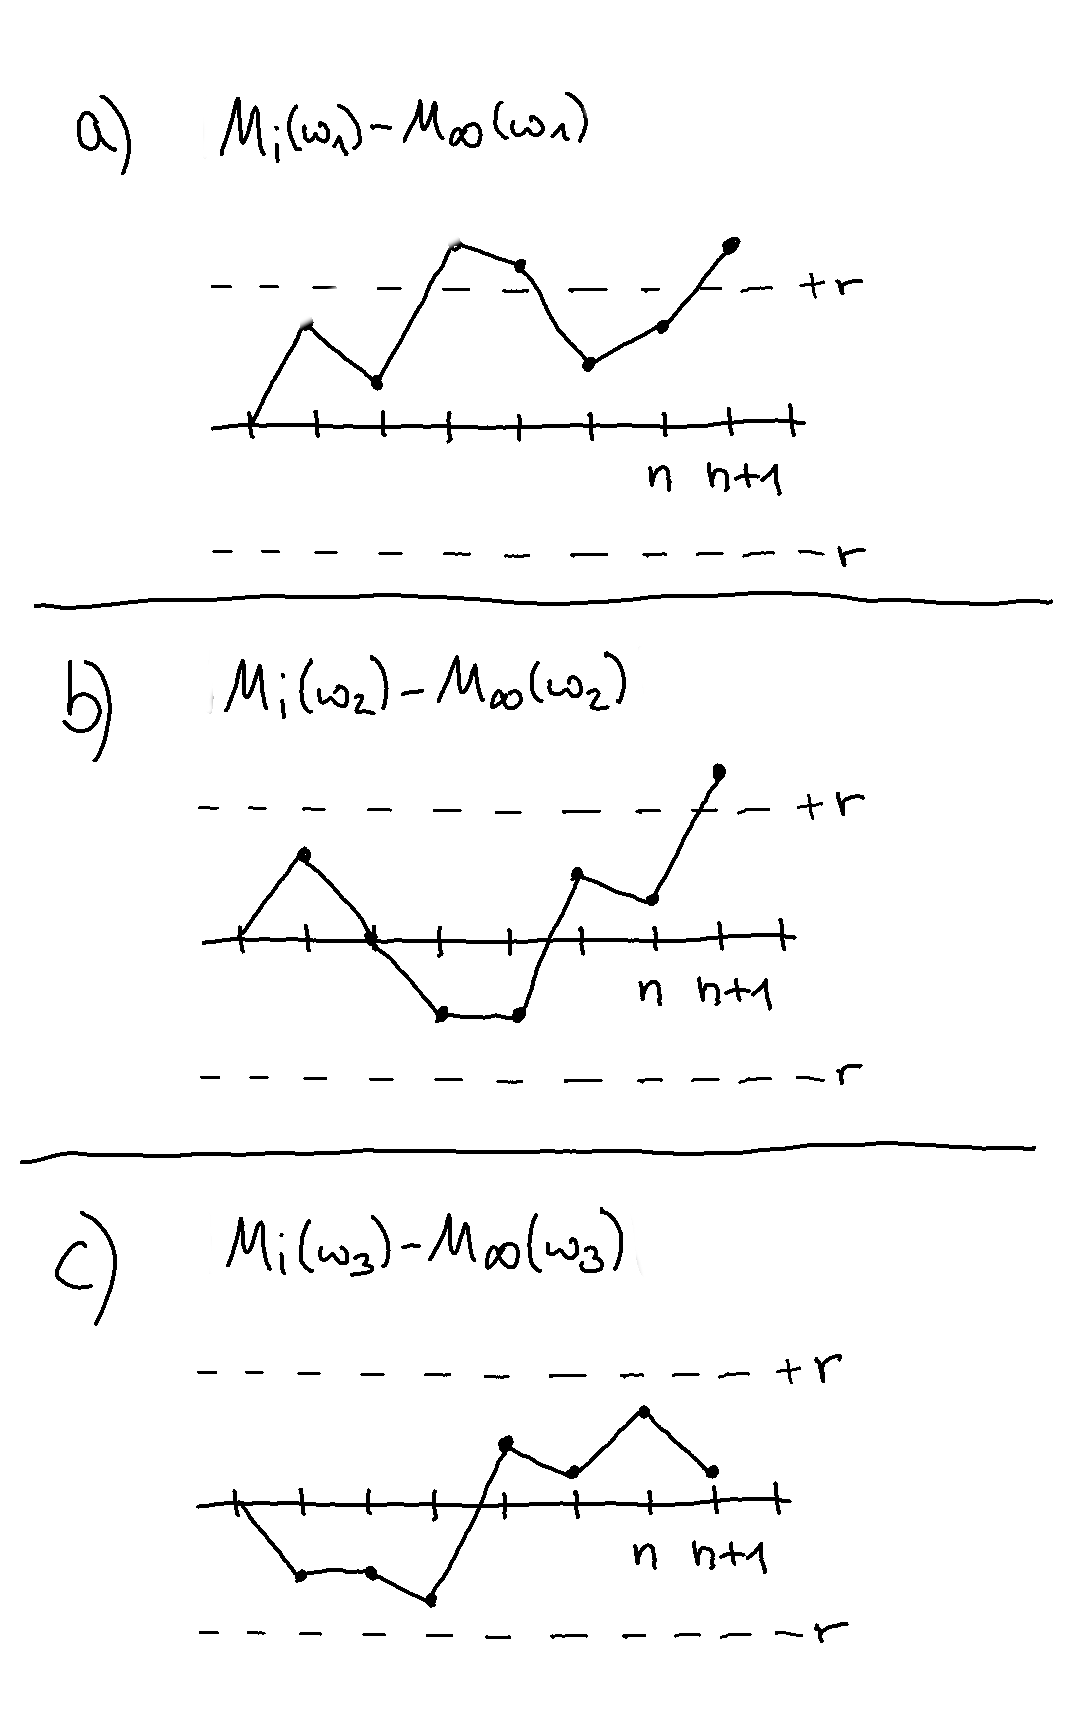
\includegraphics[width=0.65\textwidth]{\pathPrefix pics/SketchUE1.png}
		\begin{enumerate}[label=Fall \alph{*})]
			\item \qquad $\omega_1 \in A_n \quad \rightarrow\quad \omega_1 \in A_{n+1}$
			\item \qquad $\omega_2 \not\in A_n \quad \rightarrow \quad \omega_2 \in A_{n+1}$
			\item \qquad $\omega_3 \not\in A_n \quad \rightarrow \quad \omega_3 \not\in A_{n+1}$
		\end{enumerate}
		$\omega \in A_n \quad \rightarrow \quad \omega \not\in A_{n+1} \quad$ nicht möglich $\implies A_n \subset A_{n+1} \quad\forall n\in\N$
		\label{AbbUEProzess}
	\end{center}
\end{figure}

\begin{proof}[Beweis vom Professor]\enter
	$|M_n|$ ist Submartingal. Aus 4.2 folgt:
	\begin{align*}
		\exists M_\infty\in L_1:\P\left(\limn M_n=M_\infty\right)=1
	\end{align*}
	Mit Fatou kann man zeigen:
	\begin{align*}
		\E\Big[|M_\infty|^p\Big]
		&=\E\left[\limn |M_n|^p\right]
		\overset{\text{Fatou}}{\leq}
		\liminf\limits_{n\to\infty}\E\Big[|M_n|^p\Big]\leq B<\infty\\
		&\implies M_\infty\in L_p
	\end{align*}
	Jetzt nutzen wir majorierte Konvergenz:
	\begin{align*}
		\big|M_n-M_\infty\big|^p
		&\leq
		2^{p-1}\cdot\Big(|M_n|^p+|M_\infty|^p\Big)\\
		&\leq 2^{p-1}\cdot\Bigg(\left(\sup\limits_{n\in\N_0}|M_n|\right)^p+\underbrace{|M_\infty|^p}_{\text{integrierbar}}\Bigg)
	\end{align*}
	Mit Doobs $L_p$-Ungleichung folgt:
	\begin{align*}
		\left\Vert\sup\limits_{0\leq n\leq N}|M_n|\right\Vert_p
		&\leq \frac{p}{p-1}\cdot\Vert M_n\Vert_p\leq B\\
		\implies
		\left\Vert\sup\limits_{0\leq n\leq N}|M_n|\right\Vert_p
		&\leq B<\infty
	\end{align*}
	d.h. $|M_n-M_\infty|^p$ ist integrierbare obere Schranke. Folglich:
	\begin{align*}
		\limn\E\left[|M_n-M_\infty|^p\right]	
		\overset{\text{domKonv}}=
		\E\left[\limn|M_n-M_\infty|^p\right]=0
	\end{align*}
\end{proof}

